\documentclass{article}
\usepackage{tikz}
\usetikzlibrary{arrows, positioning, math, calc, mindmap}

\definecolor{mybrown}{rgb}{0.47,0.39,0.01}

\begin{document}
    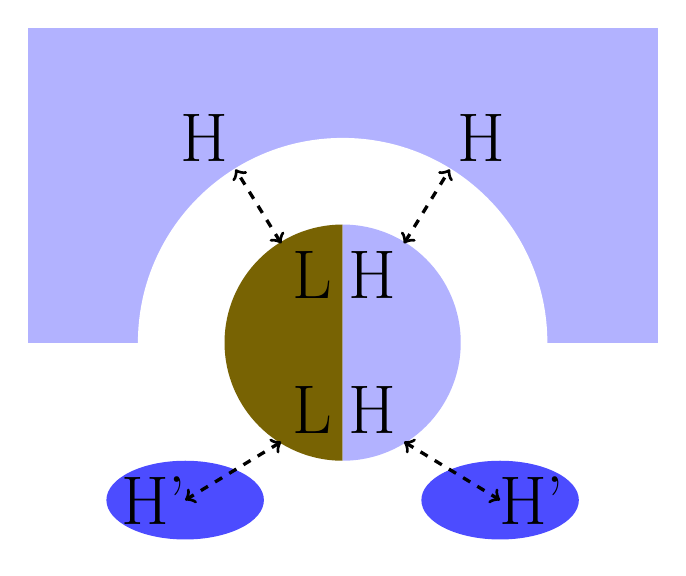
\begin{tikzpicture}[scale=2.0]
        \fill[fill=blue!30] (-2,2) rectangle (2,0);
        \fill[fill=white] (0,0) circle (1.3);
        \fill[fill=mybrown] (0, 0.75) arc (90:270:0.75);
        \fill[fill=blue!30] (0, -0.75) arc (-90:90:0.75);
        \coordinate[] (H1) at (0.39, 0.63);
        \coordinate[] (H2) at (0.68, 1.10);
        \draw[<->, dashed,very thick] (H1) --(H2);
        \node[] at ($(H1) + (-0.2, -0.2)$) {\Huge H};
        \node[] at ($(H2) + (+0.2, +0.2)$) {\Huge H};
        \coordinate[] (L1) at (-0.39, 0.63);
        \coordinate[] (H3) at (-0.68, 1.10);
        \draw[<->, dashed, very thick] (L1) --(H3);
        \node[] at ($(L1) + (+0.2, -0.2)$) {\Huge L};
        \node[] at ($(H3) + (-0.2 ,+0.2)$) {\Huge H};
        \coordinate[] (HS1) at (+1.0, -1.0);
        \coordinate[] (HS2) at (-1.0, -1.0);
        \coordinate[] (L2) at (-0.39, -0.63);
        \coordinate[] (H4) at (+0.39, -0.63);
        \fill[fill=blue!70] (HS1) ellipse (0.5 and 0.25);
        \fill[fill=blue!70] (HS2) ellipse (0.5 and 0.25);
        \draw[<->, dashed, very thick] (H4) --(HS1);
        \draw[<->, dashed, very thick] (L2) --(HS2);
        \node[] at ($(L2) + (+0.2, +0.2)$) {\Huge L};
        \node[] at ($(H4) + (-0.2 ,+0.2)$) {\Huge H};
        \node[] at ($(HS1) + (+0.2, 0)$) {\Huge H'};
        \node[] at ($(HS2) + (-0.2 ,0)$) {\Huge H'};
    \end{tikzpicture}
\end{document}
